\section{训练中期}
仿真实验开始一段时间后,Q表中各状态-动作组合都完成了至少一次更新,学习鼠的训练进入中期。

图\ref{figure_midheatmap}展示了训练进入中期后任意$1~min$内学习鼠与规则鼠的运动热点图和轨迹。与图\ref{figure_roboticheatmap}相比,这一时期的学习鼠更加“活跃”,能够较频繁地改变自身未知,并与机器鼠活动更加一致,例如,在图中的$11\sim39~s$内,两者均在同一角落附加活动,并能够逐渐进行部分行为交互。
\begin{figure}[htbp]
  \vspace{13pt}
  \centering
  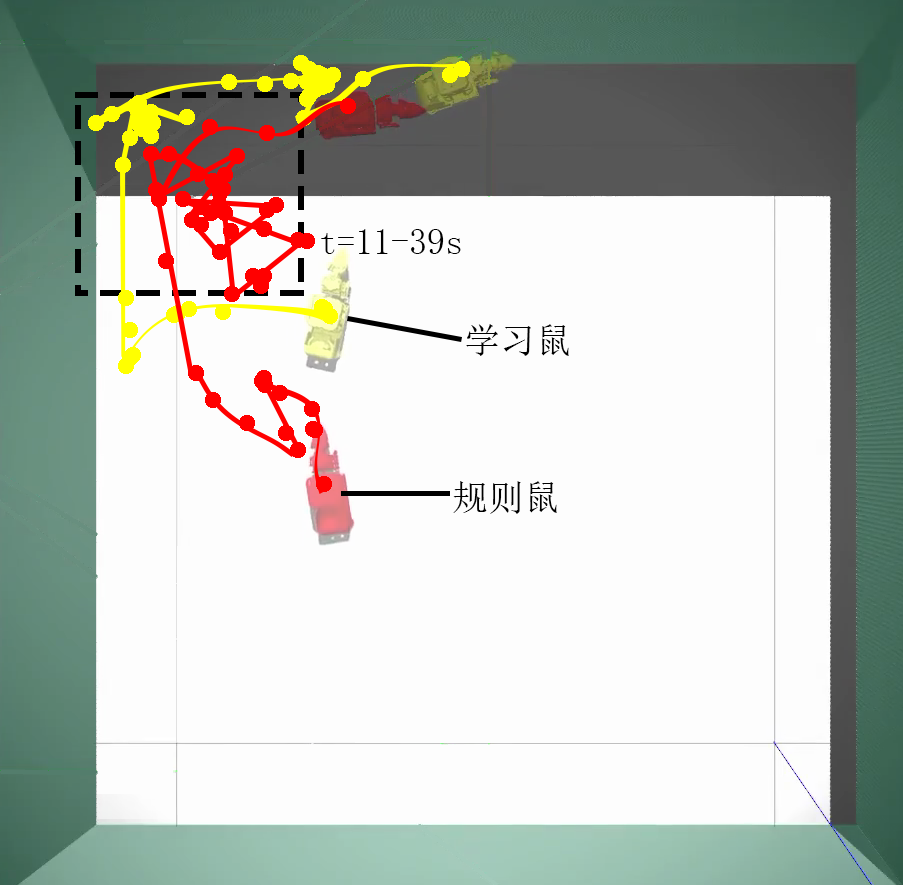
\includegraphics[height=6cm]{images/ch05/midterm/heatmap.png}
  \caption{训练中期机器鼠运动热点图及运动轨迹($1~min$)}\label{figure_midheatmap}
\end{figure}

这一阶段两者距离变化更频繁。图\ref{figure_middistance}展示期间了$1~min$内$d_{cc}$的变化情况。该图表明,在进入训练中期后,学习鼠能够更频繁地进入与规则鼠开展有效交互地距离范围($13\sim22~s$,$35\sim39~s$和$27\sim29~s$等),这表明了学习鼠已经学习到部分有利于行为交互的规则。
\begin{figure}[htbp]
  \vspace{13pt}
  \centering
  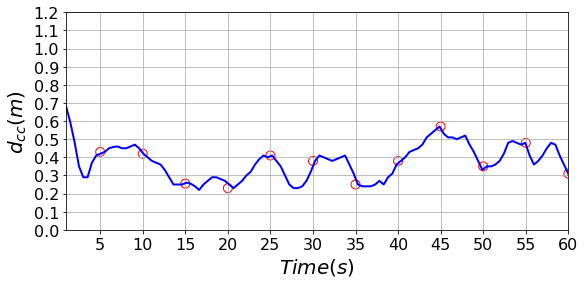
\includegraphics[height=6cm]{images/ch05/midterm/distance.png}
  \caption{训练中期机器鼠中心距离($1~min$)}\label{figure_middistance}
\end{figure}

但即便两者距离足够近,也并不意味着能够开展有效的行为交互。以图\ref{figure_middistance}中$35\sim39~s$这一时间段为例,如图\ref{figure_mid35-39}所示,规则鼠始终在学习鼠右侧活动,此时学习鼠虽然产生了梳理等一些试图交互的动作,但由于并未面对交互伙伴,因此规则鼠并未作出回应,只是在不断地靠近和远离学习鼠中切换。
\begin{figure}[htbp]
  \vspace{13pt}
  \centering
  \subfigure[$t=35~s$]{\label{figure_midt69}
  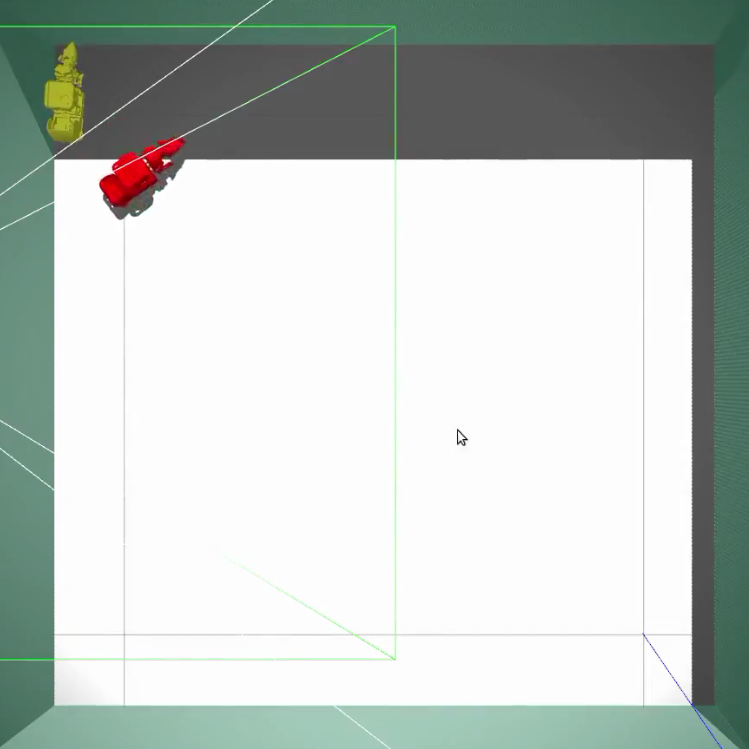
\includegraphics[height=2.5cm]{images/ch05/midterm/t69.png}
  }
  \subfigure[$t=36~s$]{\label{figure_midt72}
  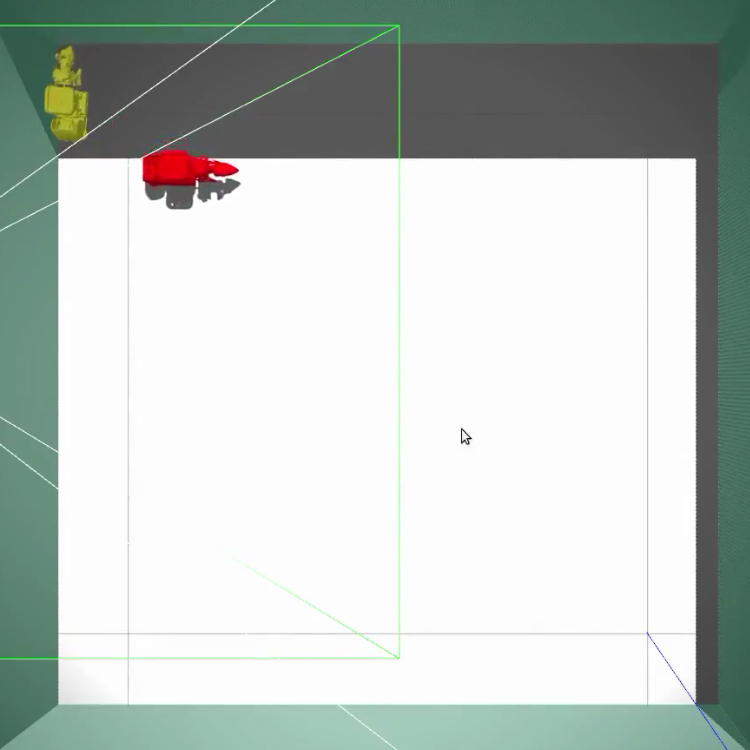
\includegraphics[height=2.5cm]{images/ch05/midterm/t72.png}
  }
  \subfigure[$t=37~s$]{\label{figure_midt75}
  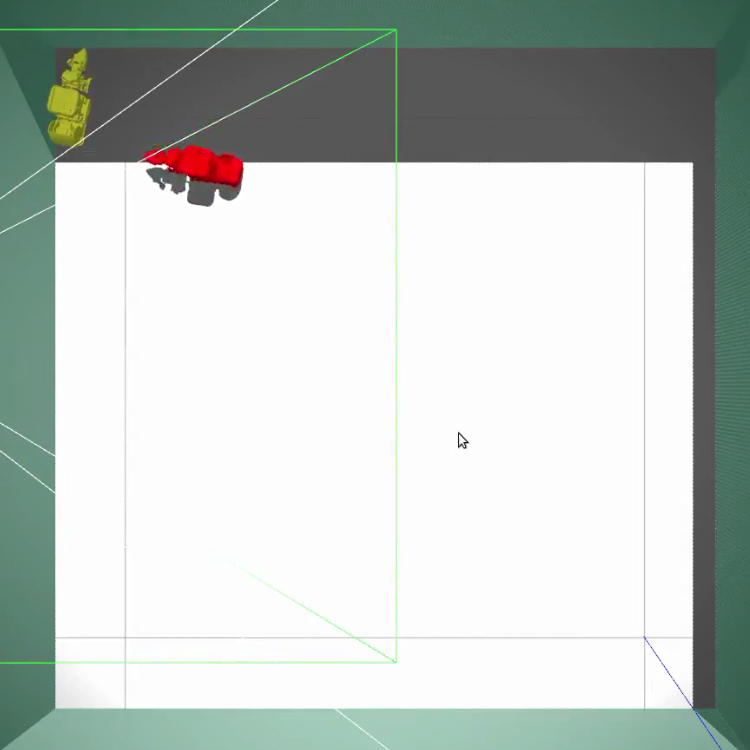
\includegraphics[height=2.5cm]{images/ch05/midterm/t75.png}
  }
  \subfigure[$t=38~s$]{\label{figure_midt77}
  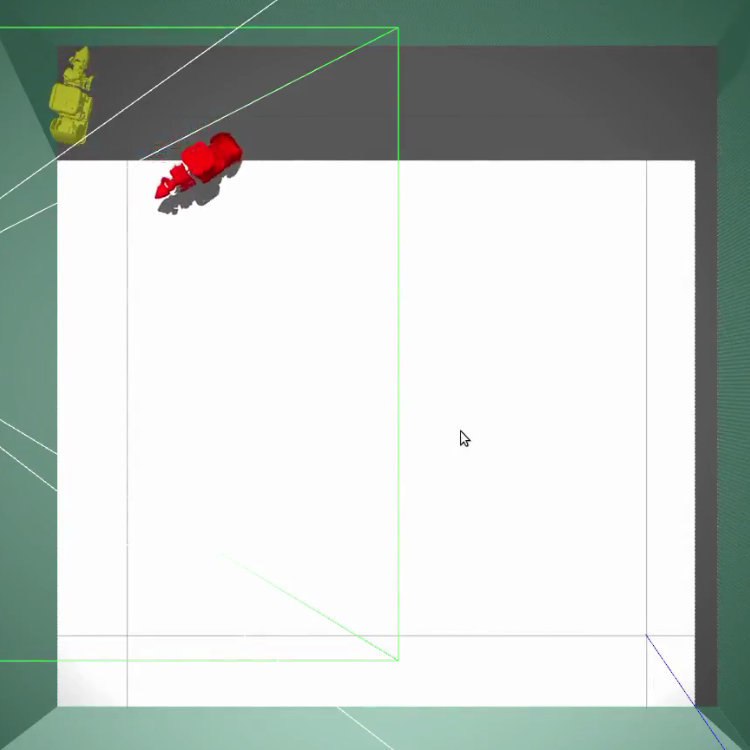
\includegraphics[height=2.5cm]{images/ch05/midterm/t77.png}
  }
  \caption{训练中期$35\sim39~s$内学习鼠与规则鼠动作表现}\label{figure_mid35-39}
\end{figure}

这一阶段学习鼠行为的另一特点是试错(trial-and-error search),在图\ref{figure_midheatmap}中,学习鼠长时间停留在墙角便是如此。图\ref{figure_actioncnt}统计了这一时段学习鼠各动作的执行频次,其中浅绿色$s_4$(右转)为理论上其应当执行的最优动作,数据表明这一动作的执行次数明显低于其他动作,而$s_3$(左转)执行次数较多。这是由于前期错误经验的积累,当学习鼠观测到环境处于某一状态时,根据尚不完善的Q表做出错误的决定,因此需要在不断地错误尝试中积累负向奖励,直到这些非最优的状态-动作组Q值低于最优状态-动作组。同样由于强化学习奖励的延时性,负向奖励需要一定时间才能传递到特定状态-动作组,因此试错所需时间较长。
\begin{figure}[htbp]
  \vspace{13pt}
  \centering
  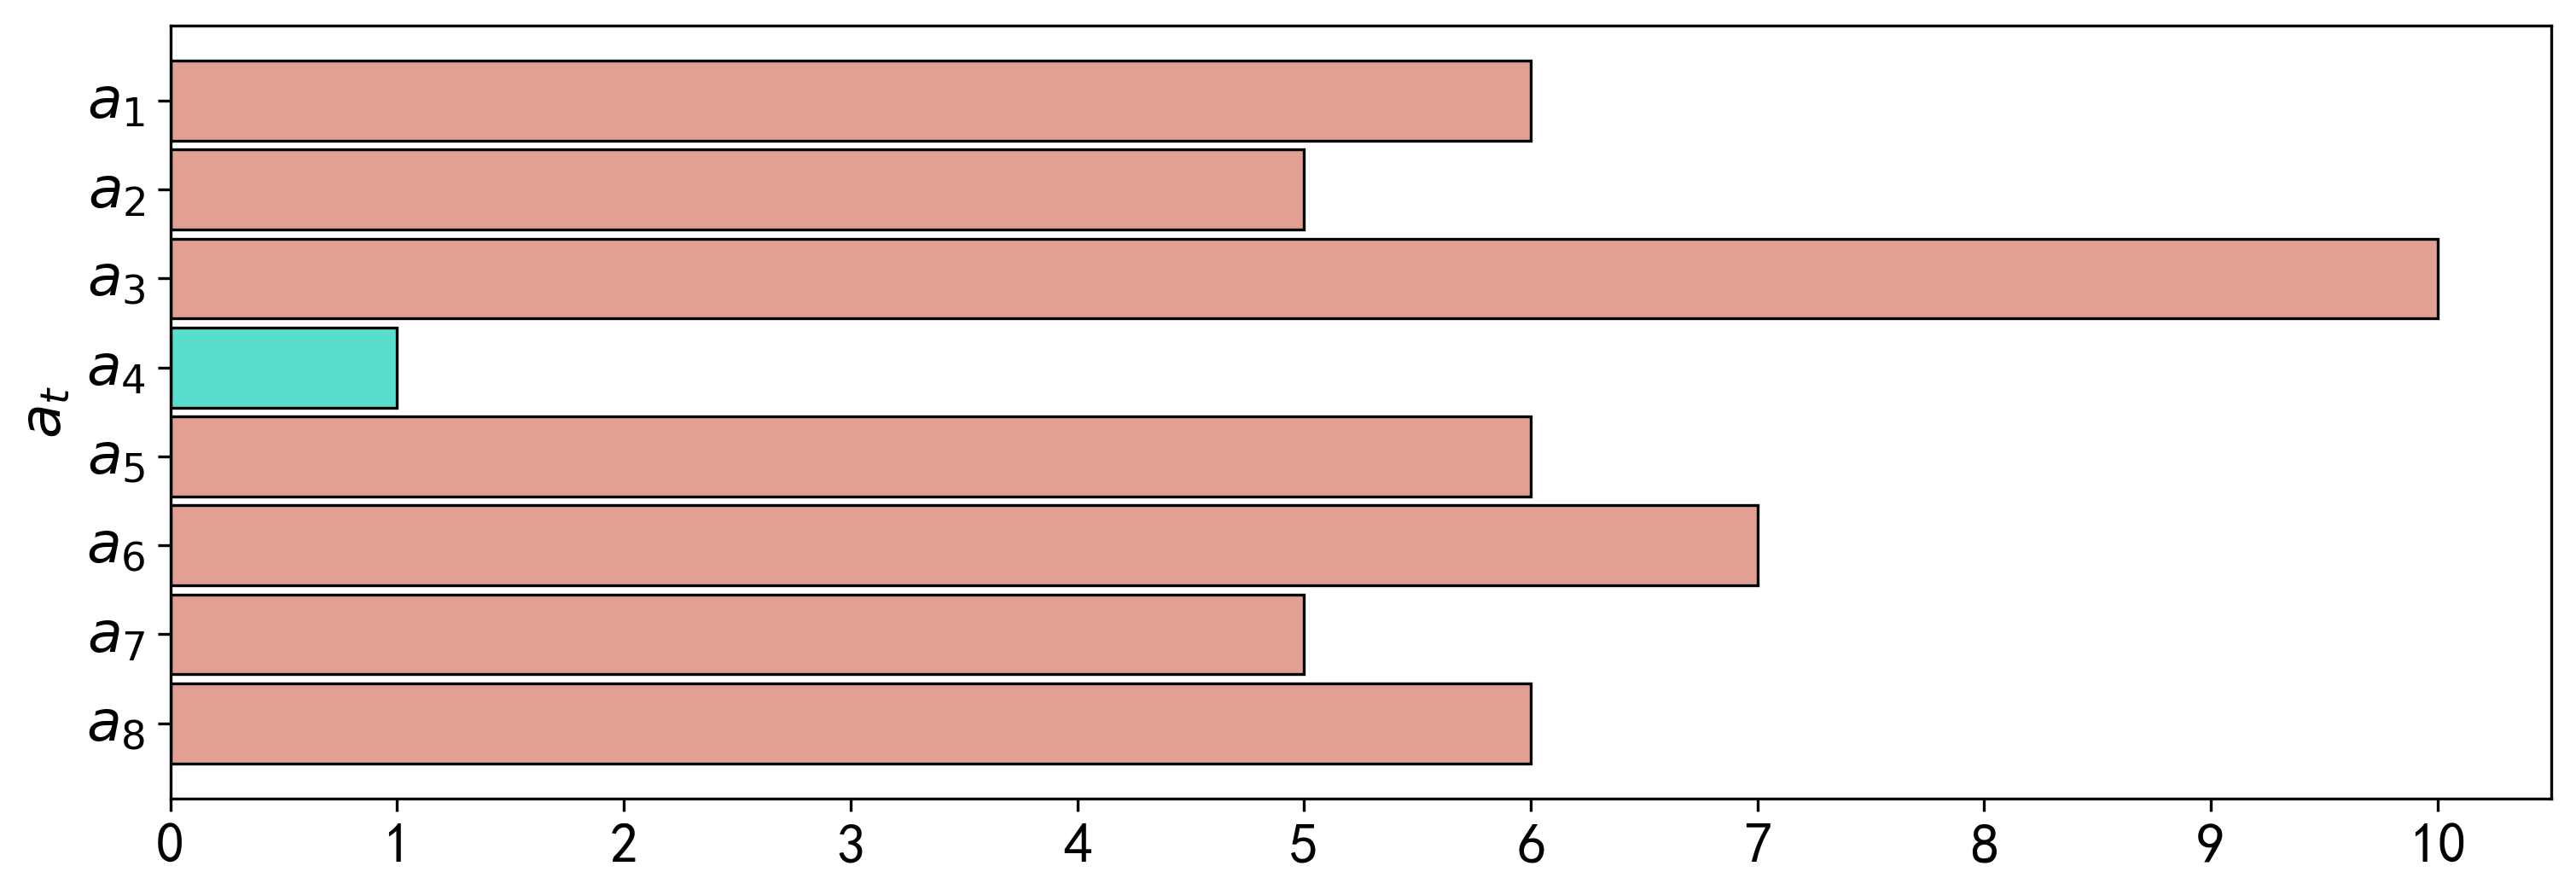
\includegraphics[height=4cm]{images/ch05/midterm/actioncnt.png}
  \caption{学习鼠在墙角时动作执行频次}\label{figure_actioncnt}
\end{figure} 